



%\begin{frame}{Proyectos de Investigación}
\begin{frame}{\citetitle{MarcoNuno_Revista_2020_04_00} \footnotemark (1)}
\begin{columns}
\begin{column}{0.70\textwidth}
Propuesta:
		\begin{itemize}
		\item Un \textit{Cariograma} es una representación ordenada de los cromosomas.  
		\item Un \textit{Citogenetista} es una experto que diagnotisca enfermedades genéticas a partir de Cariograma.		
		\item Un sistema que auxilie al Citogenetista a crear el Cariograma de forma automática.
		\item Se requieren técnicas de visión por computadora y aprendizaje automáticos.
		\end{itemize}
\end{column}
\begin{column}{0.30\textwidth}  
    \begin{center}
     %%%%% this is a minipage, so \textwidth is already adjusted to the size of the column
     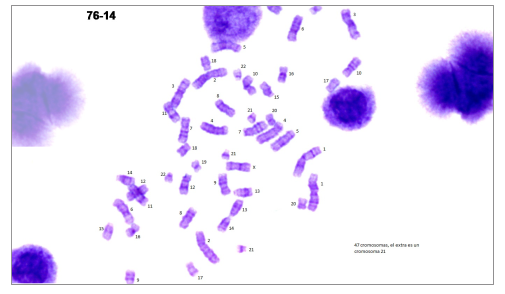
\includegraphics[width=0.98\textwidth]{Figs/Karyogram1}
     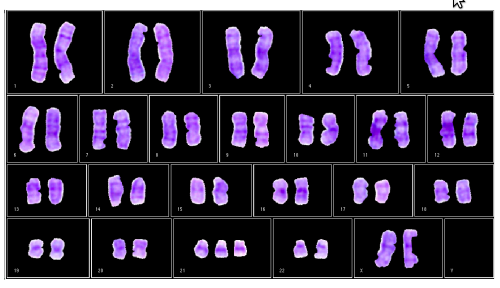
\includegraphics[width=0.98\textwidth]{Figs/Karyogram2}
     \end{center}
\end{column}
\end{columns}
\footnotetext[1]{\fullcite{MarcoNuno_Revista_2020_04_00}}
\setcounter{footnote}{0}
\end{frame}


\begin{frame}{\citetitle{MarcoNuno_Revista_2020_04_00} \footnotemark (2)}
\begin{columns}
\begin{column}{0.6\textwidth}
Pasos a aplicar:
		\begin{enumerate}
		\item Segmentación de los cromosomas individuales 
		\item Extracción de características
		\item Clasificación por tamaño
		\item Clasificación por tipo dentro de cada tamaño
		\item Integración
		\item Construcción del Cariograma
		\end{enumerate}
    \begin{center}
     %%%%% this is a minipage, so \textwidth is already adjusted to the size of the column
     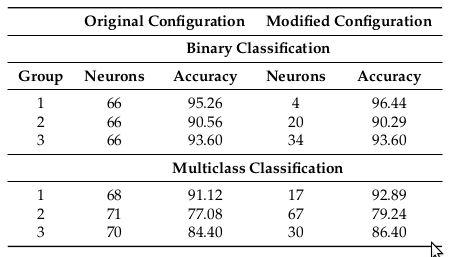
\includegraphics[width=0.5\textwidth]{Figs/Karyogram4}
     \end{center}


\end{column}
\begin{column}{0.4\textwidth}  
    \begin{center}
     %%%%% this is a minipage, so \textwidth is already adjusted to the size of the column
     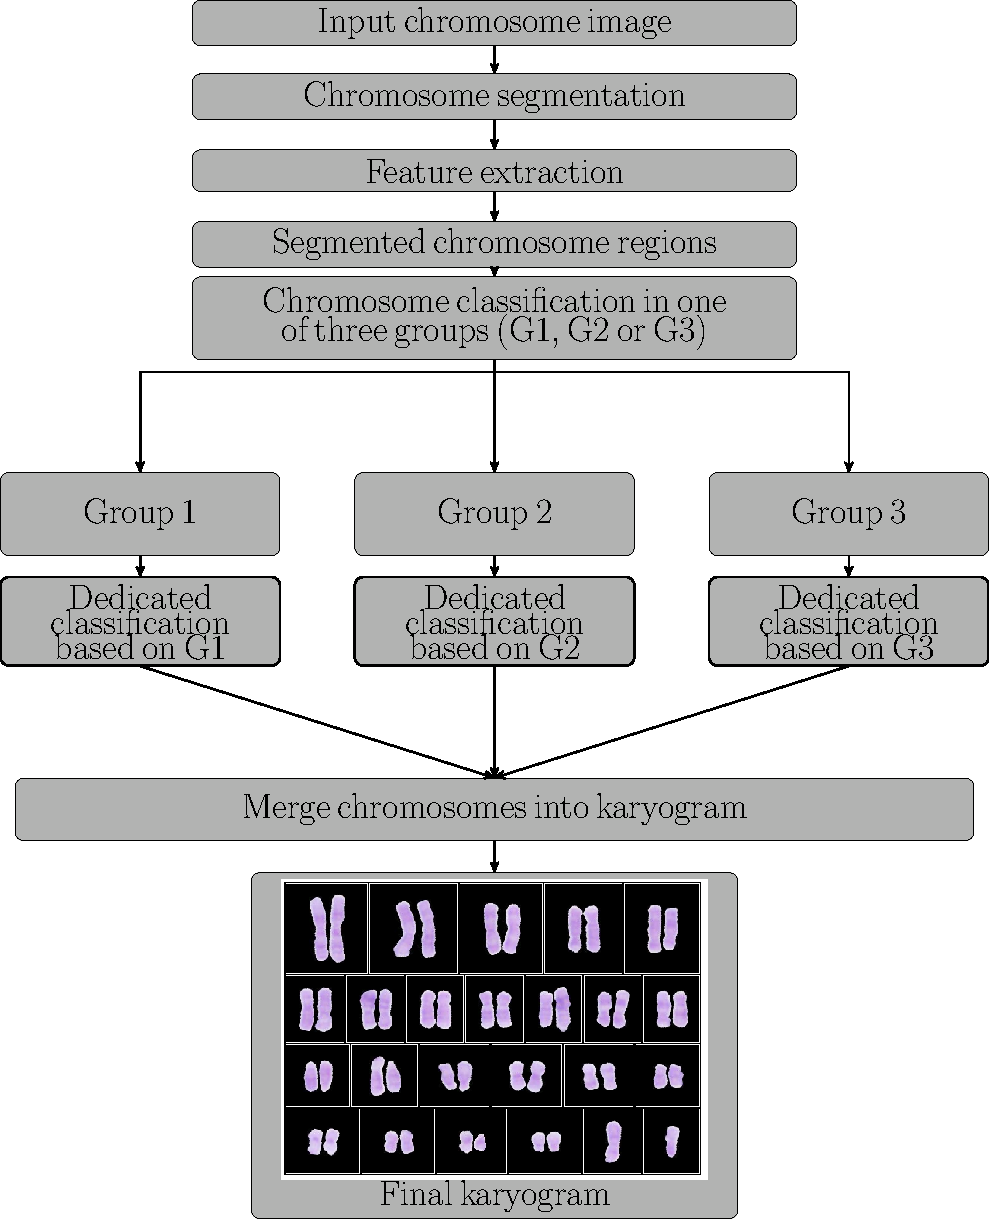
\includegraphics[width=0.7\textwidth]{Figs/Karyogram5}
     \end{center}
\end{column}
\end{columns}
\end{frame}






